%\section{Hardware}\label{sec:hardware}
%This section provides a brief overview of the hardware used in the cart pendulum setup.
%
\section{Motors}\label{sec:motors}
There are two Maxon 370356 brushed DC motors, see \autoref{fig:maxonMotor}, used in the setup.\cite{maxonMotor}

\begin{figure}[H]
  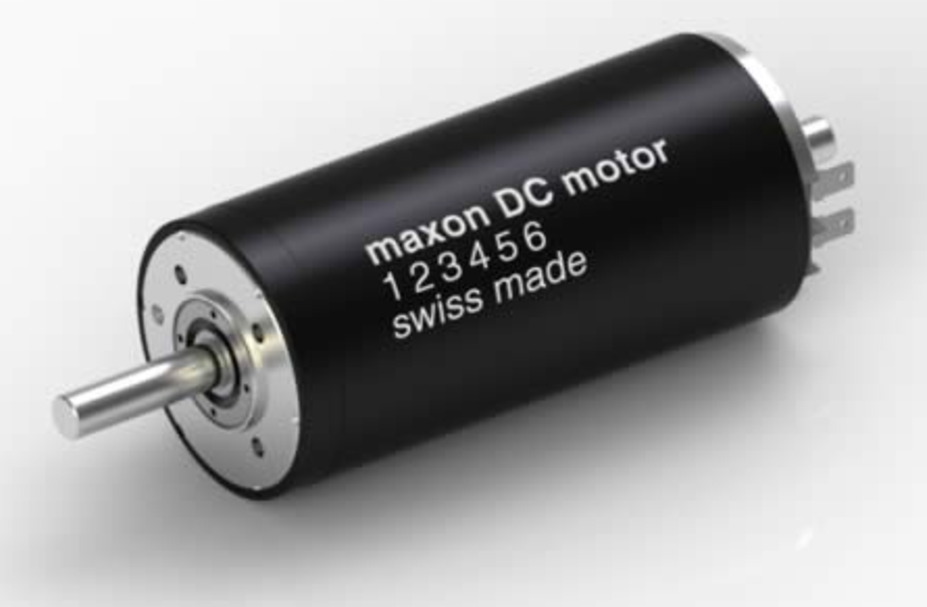
\includegraphics[width=.26\textwidth]{figures/maxonMotor}
  \caption{The motor used in the setup.\cite{maxonMotor}}
  \label{fig:maxonMotor}
\end{figure}

The most interesting characteristic of the maxon motor for the purposes of this report are shown in \autoref{table:motorParameters}.

\begin{table}[H]
  \begin{tabular}{|l|l|l|}
    \hline %--------------------------------------------------------------------------------------
    \textbf{Characteristic}                    & \textbf{Quantity} & \textbf{Unit}              \\
    \hline %--------------------------------------------------------------------------------------
    Nominal torque (max. continuous torque)    & \SI{420e-3}       &  \si{N \cdot m}            \\
    \hline %--------------------------------------------------------------------------------------
    Nominal current (max. continuous current)  & \SI{4.58}         &  \si{A}                    \\
    \hline %--------------------------------------------------------------------------------------
    Torque constant                            & \SI{93.4e-3}      &  \si{N\cdot m\cdot A^{-1}} \\
    \hline %--------------------------------------------------------------------------------------
    Rotor inertia                              & \SI{54.2e-6}      &  \si{kg\cdot m^2}          \\
    \hline %--------------------------------------------------------------------------------------
    Weight                                     & \SI{1.1}          &  \si{kg}                   \\
    \hline %--------------------------------------------------------------------------------------
  \end{tabular}
  \caption{Motor characteristics given by \cite{maxonMotor}.\label{table:motorParameters}}
\end{table}

One of the motors is mounted on a pulley driving the belt, see \autoref{fig:systemSetup}. The other motor is disabled and acts only as a bearing at the pendulum pivot point.

\section{Motor Encoders}

Each of the two motors are equipped with an HEDS 5540 optical quadrature encoder, see \autoref{fig:maxonMotor}. The moment of inertia added by the encoder is negligibly small at only \SI{0.6e-6}{kg\cdot m^2} and is not mentioned further in this report.\cite{avagoTechnologies}
%
\begin{figure}[H]
  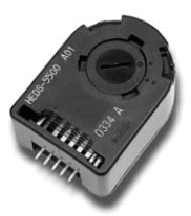
\includegraphics[width=.16\textwidth]{figures/infineonEncoderHEDS5540-A14}
  \caption{The encoders used in in this project. \cite{avagoTechnologies}}
  \label{fig:encoder}
\end{figure}

\section{Motor Controller}
Two Maxon ADS 50/10 motor controllers, see \autoref{fig:maxonMotorController}, are mounted on the cart pendulum setup. One on the side to control the driving motor and the other, not used in this project, mounted on the cart. The datasheet states that the motor controller weights \SI{0.38}{kg}, but again, since the remaining mass of the cart is unknown and can not be measured, the cart mass must be estimated.\cite{maxonMotorController}
%
\begin{figure}[H]
  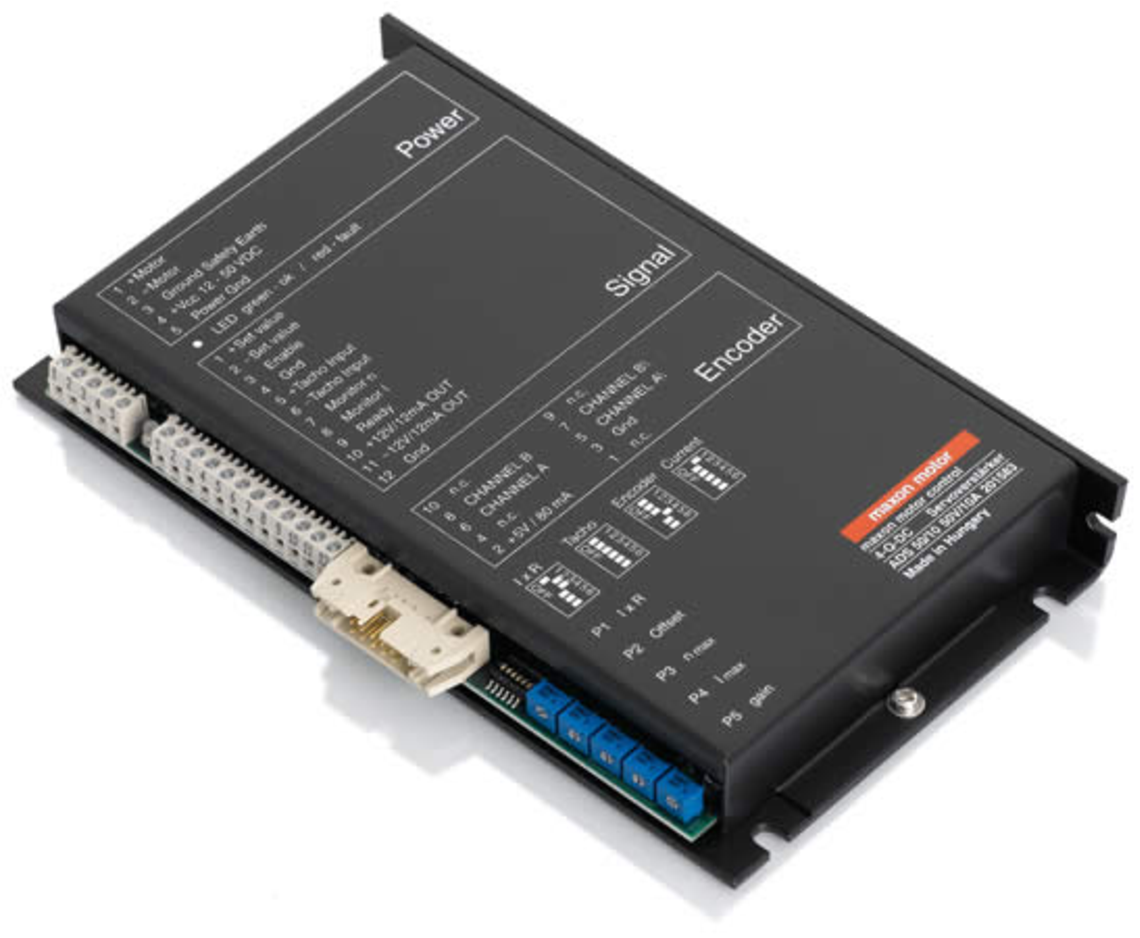
\includegraphics[width=.26\textwidth]{figures/maxonMotorController}
  \caption{The Maxon motor controller used in the setup.\cite{maxonMotorController}}
  \label{fig:maxonMotorController}
\end{figure}

The motor controller can be configured in four different modes, \cite{maxonMotorController}
\vspace{-10pt}
\begin{itemize}
  \item[-] Speed control using tacho signals
  \item[-] Speed control using encoder signals
  \item[-] IxR compensated speed control
  \item[-] Torque or current control
\end{itemize}
\vspace{-10pt}
The first three modes are forms of speed control while the last is current control relating directly to torque and thereby also force on the belt. The chosen mode for this project is therefore current control. The conversion from armature current to motor torque is by use of the torque constant given in \autoref{table:motorParameters}. To set the armature current the motor controller requires a $\pm$\SI{10}{V} input signal \cite{maxonMotorController}. This input is provided through a shield from the microcontroller, so the conversion to armature current is handled in the following.\fxnote{source}

\section{Micro Controller}
The control design is implemented on a Teensy 3.6 microcontroller, see \autoref{fig:teensy3_6}, provided in the setup. The armature current reference is provided through one of the microcontroller's two 12 bit DAC's (Digitl-to-Analog Converter) placed on an external pin of the microcontroller. The Teensy 3.6 runs on \SI{3.3}{V} provided by an onboard regulator from \SI{5}{V} USB supply, and so the analog output is in the range of $0-$\SI{3.3}{V} with a 12 bit resolution.\cite{teensyDataSheet}\\
The motor encoders are decoded on the shield, see next section, and read through an 8 bit parallel data bus by the microcontroller.

\begin{figure}[H]
  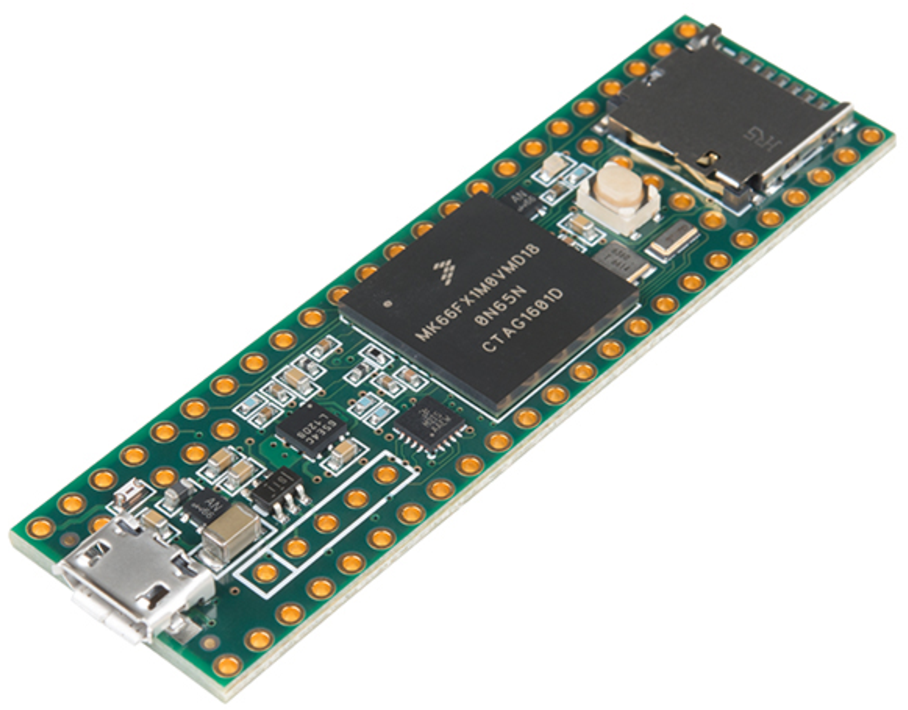
\includegraphics[width=.2\textwidth]{figures/teensy3_6}
  \caption{The teensy 3.6 used as main control unit in the setup. \cite{sprkfunTeensy}}
  \label{fig:teensy3_6}
\end{figure}

The Teensy 3.6 uses a bootloader which allows programming through USB using the Teensyduino add-on for the Arduino IDE.\cite{sprkfunTeensy}

\section{Shield}
A shield located by the microcontroller handles conversion/interfacing between the microcontroller and the setup. The motor encoders are decoded using Avago HCTL-2021-PLC decoders, mounted on the shield, which outputs 2000 ticks pr. revolution.\cite{avagoDataSheet} This results in a resolution of $2\pi/2000=$ \SI{\pi e-3} rad/tic, for the pendulum angle, $\theta$, and $2\pi r /2000=\nolinebreak 2\pi\cdot 0.028 /2000\approx$ \SI{0.088e-3} m/tic for the position along $x$.
The armature current reference is provided from the microcontroller which as mentioned outputs $0-$\SI{3.3}{V} while the motor controller requires a $\pm$\SI{10}{V} input. This is handled by an amplification on the shield converting the $0-$\SI{3.3}{V} to the required $\pm$\SI{10}{V}.
A previous project group has tested the relation between armature current and different 12 bit values from the micro controller. The test was conducted using a current clamp and an oscilloscope to measure the armature current in the motor. By linear regression they arrived at the following relation,
%
\begin{flalign}
  \text{bit}_\text{DAC} &= 105.78 \cdot i_{a} + 1970  \ \ \ . & 
  \label{eq:Ia-bit}
\end{flalign}
%
An other way of measuring the current is from an output directly on the motor controller. It is found that this output is slightly different than the current measured directly over the motor using a current clamp. It is difficult to know if the torque constant supplied by the company is matched using one or the other way of measuring. So a test is conducted to verify \autoref{eq:Ia-bit}, in which the steady state hold force is measured directly on the cart using a luggage scale as an alternative Newton-meter. The results of the force test are seen in \autoref{fig:forceTest1} and \ref{fig:forceTest2}. % and a test journal is provided in \fxnote{refference appendix}.

\begin{figure}[H]
  \hspace{-10pt}
  \captionbox
  {
    Result of force test compared to theoretical result with current model.
    \label{fig:forceTest1}
  }
  {
    %\hspace{-1cm}
    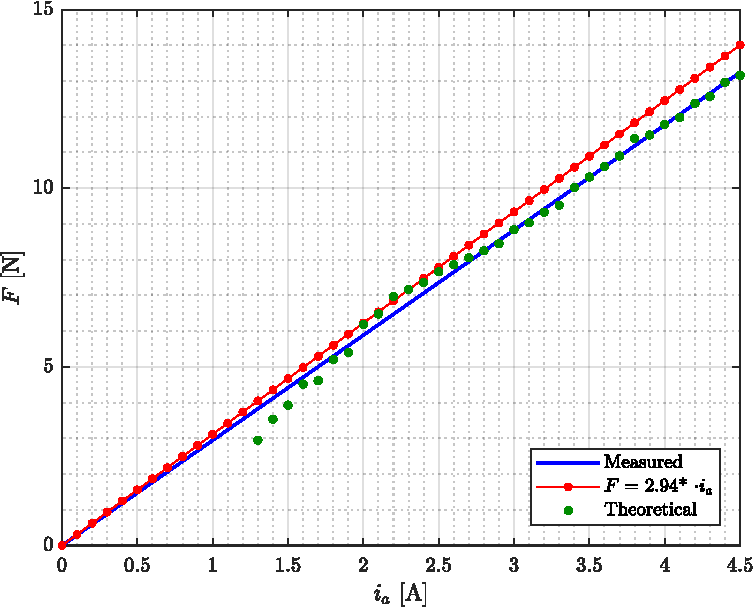
\includegraphics[width=.45\textwidth]{figures/forceTest1}%\vspace{-11pt}
  }
  \hspace{20pt}
  \captionbox
  {
    Showing how the corrected model for $i_a$ now fits exactly the results of the force test.
    \label{fig:forceTest2}
  }
  {
    %\hspace{-1cm}
    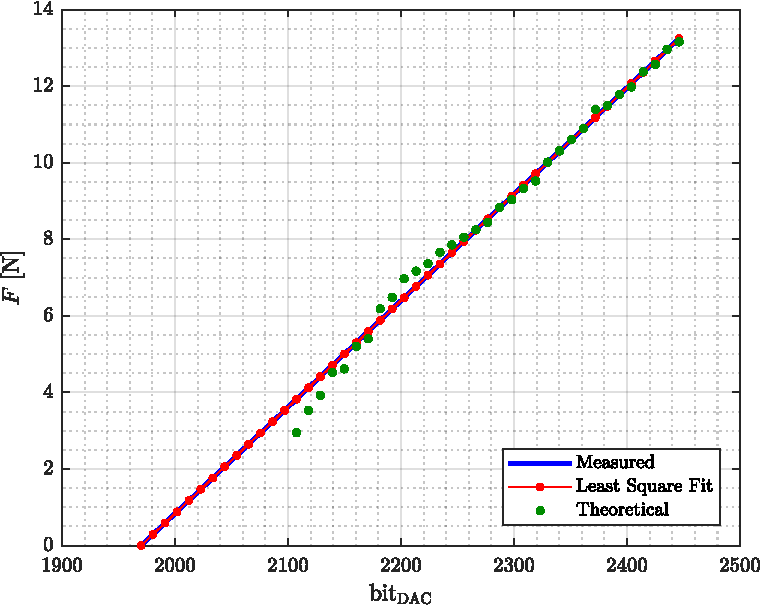
\includegraphics[width=.45\textwidth]{figures/forceTest2}\vspace{6pt}
  }  
\end{figure}

The measurements should be more correct at higher forces since friction then causes less disturbance in the measurements. However, no measurements are excluded in the regression as it is noted that the regression line fits the upper part of the data very well. Measurements lower than $F = 2.95$ were considered unreliable due to friction and therefore not included in the data-set.
In \autoref{fig:forceTest1} the armature current is scaled using \autoref{eq:Ia-bit} and the theoretical line is calculated using that $F = \tfrac{1}{r} k_\tau i_a$. As the theoretical line does not coincide exactly with the least square regression, \autoref{eq:Ia-bit} is tweaked so that,
\begin{flalign}
  \text{bit}_\text{DAC} &= 111.9 \cdot i_{a} + 1970  \ \ \ , & 
  \label{eq:Ia-bit-corrected}
\end{flalign}
which leads to the result seen in \autoref{fig:forceTest2}, where the theoretical line now coincide with the least square regression of the measurement data.
